\documentclass[a4paper]{article}

\usepackage[utf8]{inputenc}
\usepackage[portuguese]{babel}
\usepackage{a4wide}
\usepackage[pdftex]{hyperref}
\usepackage{graphicx}
\usepackage{wrapfig}
\usepackage{amsmath}
\usepackage{verbatim}
\usepackage{caption}
\usepackage{subcaption}
\usepackage{float}
\usepackage{listings} 
\usepackage{color}

\definecolor{codegreen}{rgb}{0,0.6,0}
\definecolor{codegray}{rgb}{0.5,0.5,0.5}
\definecolor{codepurple}{rgb}{0.58,0,0.82}
\definecolor{backcolour}{rgb}{0.95,0.95,0.92}
\definecolor{white}{rgb}{1,1,1}

\lstdefinestyle{mystyle}{
    backgroundcolor=\color{backcolour},   
    commentstyle=\color{codegreen},
    keywordstyle=\color{magenta},
    numberstyle=\tiny\color{codegray},
    stringstyle=\color{codepurple},
    basicstyle=\footnotesize,
    breakatwhitespace=false,         
    breaklines=true,                 
    captionpos=b,                    
    keepspaces=true,                 
    numbers=left,                    
    numbersep=5pt,                  
    showspaces=false,                
    showstringspaces=false,
    showtabs=false,                  
    tabsize=2
}
 
\lstset{style=mystyle}


\begin{document}

\begin{titlepage}
\begin{center}



\includegraphics[width=0.6\textwidth]{logo.jpg}\\[0.5cm]

{\large Universidade do Minho - Escola de Engenharia}\\[0.5cm]

{\large Processamento de Linguagens}\\[0.5cm]

% Title
\rule{\linewidth}{0.5mm} \\[0.4cm]
{ \huge \bfseries Processador de textos preanotados com Freeling\\[0.4cm] }
\rule{\linewidth}{0.5mm} \\[1.5cm]

% Author and supervisor
\noindent
\begin{minipage}{0.4\textwidth}
  \begin{flushleft} \large
    \emph{Autores :}\\
    Daniel Maia \textsc{(A77531)}\\
    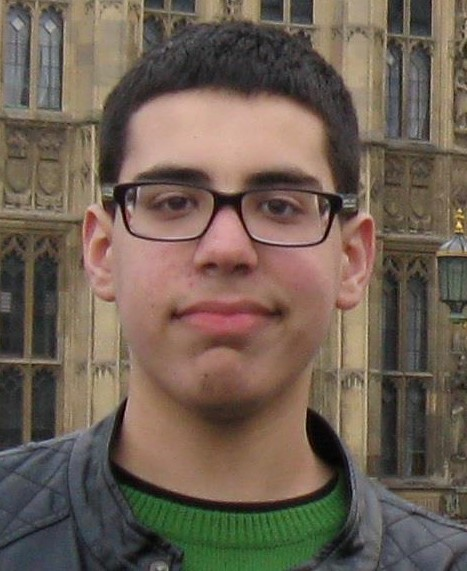
\includegraphics[width=1.5cm]{daniel.jpg}\break
    Diogo Silva\textsc{(A78034)}\\
    
\includegraphics[width=1.5cm]{afonso.jpg}\break
    Marco Silva\textsc{(A79607)}\\
    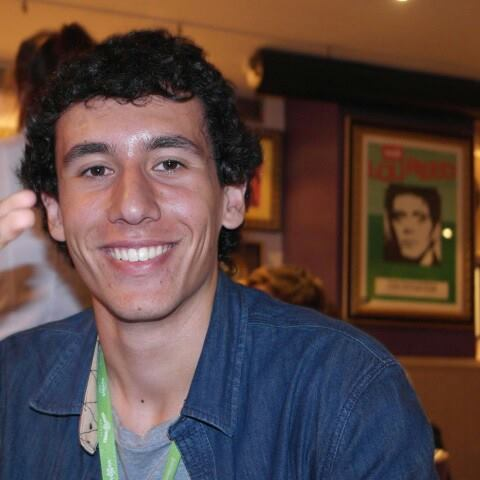
\includegraphics[width=1.5cm]{marco.jpg}\break
  \end{flushleft}
\end{minipage}%
\vfill

% Bottom of the page
{\large Versão 1.0 \\ \today}

\end{center}
\end{titlepage}


\begin{abstract}

\hspace{3mm} Este trabalho prático tem como principais objetivos:

\begin{itemize}
    \item aumentar a experiência de uso do ambiente Linux e de ferramentas de apoio à programação;
    \item aumentar a capacidade de escrever Expressões Regulares para descrição de padrões de frases;
    \item desenvolver Processadores de Linguagens Regulares;
    \item utilizar o sistema de produção para filtragem de texto \textit{Gawk}.
\end{itemize}

\par Com este intuito, serão planificados e implementados um conjunto de programas para resolver problemas envolvendo o processamento de ficheiros de texto, que requererão ao uso de cada uma destas competências. 

\par É com esta intenção que, no final do projeto, se disponha de um conjunto de programas capazes de examinar o conteúdo de um ficheiro escrito em formato Corpora \textit{Freeling}. A partir destes, será possível extrair o número de extratos que um dado ficheiro contém, gerar listas de nomes próprios, verbos, substantivos, advérbios e adjetivos de um ficheiro, calculando também o respetivo número de ocorrências de cada um, e determinar o dicionário implícito à sintaxe Corpora, analisando todas as palavras do texto.

\end{abstract}

\pagebreak
\tableofcontents

\pagebreak
\section{Introdução}
\label{sec:1}

\hspace{3mm} O \textit{AWK} é uma linguagem de programação comum em sistemas operativos \textit{Unix}, desenhada para processamento de texto e tipicamente utilizada como uma ferramenta de extração de informação. Para tal, recorre extensivamente ao tipo de dados \textit{string}, a \textit{arrays} associativos e a Expressões Regulares. \cite{Awk}

\par Um ficheiro de texto é tratado pelo \textit{AWK} como uma sequência de registos, sendo cada linha um registo. Cada linha é subdividida num conjunto de campos (\textit{fields}), separadas por um carater ou conjunto de carateres (por defeito, um ou mais espaços em branco), denominado \textit{Field Separator}, ou FS. Um programa em \textit{AWK} lê o \textit{input} um linha de cada vez, procurando padrões definidos pelo programador e, por cada padrão que encontra, executa a ação associada.\cite{Aho}

\par O \textit{Gawk} (GNU \textit{AWK}) é uma distribuição do \textit{AWK} que permite que a extensão de funcionalidades do \textit{AWK} através de bibliotecas partilhadas. Como tal, será esta a distribuição utilizada para este projeto, no qual se aplicará conhecimento para processar ficheiros de texto contendo \textit{corpora} textual, especificamente, no formato \textit{Freeling}.

\par Genericamente, os corpora agrupam textos aos quais adicionam informação de anotação frásica e morfossintática. O formato \textit{Freeling} separa extratos com uma linha em branco e usa colunas separadas por espaços para a informação morfossintática de cada palavra. As colunas presentes no contexto deste projeto são: \texttt{num, palavra, lema, pos-tag, pos} (\textit{part of speech}), \texttt{features} e \texttt{árvore}.

%------------------------------------------------------------------------

\pagebreak
\section{Descrição do Trabalho e Análise de Resultados}
\label{sec:2}

\subsection{Número de extratos}

\hspace{3mm} Para a construção da solução que determina o número de extratos foi determinante a análise prévia dos ficheiros. Deste modo, observou-se que segundo a estruturação dos ficheiros fornecidos, cada extrato encontra-se delimitado por uma linha em branco no seu final.

\begin{figure}[!h]
    \centering
    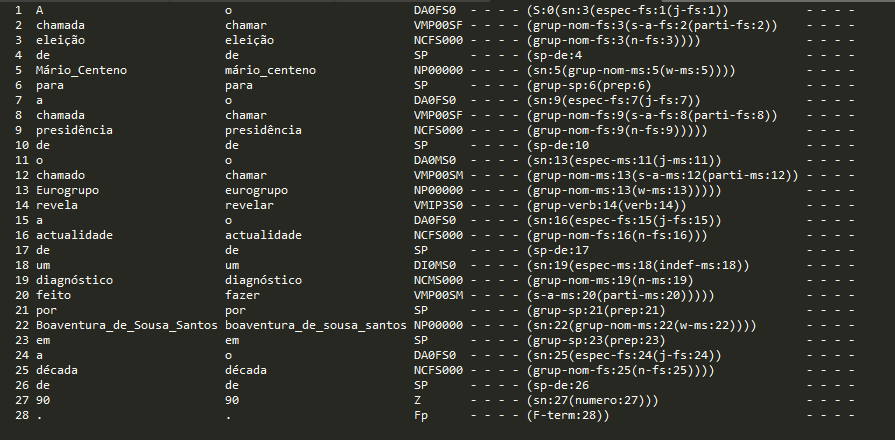
\includegraphics[width=14cm]{extrato.png}
    \caption{Extrato exemplo.}
    \label{fig:ext}
\end{figure}

\par Assim, não sendo necessário efetuar qualquer ação na secção \textit{BEGIN} do \emph{awk} ou alterar o \emph{field separator} uma vez que as linhas com informação não irão ser processadas neste contexto, procede-se apenas à definição de uma clausula. A condição desta será então o \textit{NF} (\emph{number of fields}) igual a 0, procedendo assim à contagem das linhas em branco dos ficheiros incrementando uma variável \emph{conta}.

\begin{lstlisting}[language=Awk, caption=Condição de contagem de um extrato e respetiva ação tomada.]
	NF == 0 {conta++}
\end{lstlisting}

\par No final de toda a informação ser processada, na secção \textit{END} do \emph{awk}, procede-se à devolução do valor armazenado no contador, sendo assim apresentado ao utilizador o número de extratos presentes nos ficheiros fornecidos ao \emph{awk}.

\begin{lstlisting}[language=Awk, caption=Devolução do resultado obtido.]
	END {print conta}
\end{lstlisting}

%------------------------------------------------------------------------

\subsection{Lista dos personagens do Harry Potter}

\hspace{3mm} De forma a dar utilidade à informação contida nos ficheiros \textit{harrypotter1} e \textit{harrypotter2}, que se encontram preanotados com \textit{Freeling}, tomou-se a decisão de produzir um pequeno relatório com alguma informação relacionada com as personagens presentes nos dois primeiros livros da saga, nomeadamente, \textbf{Harry Potter e a Pedra Filosofal} (HP1) e \textbf{Harry Potter e a Câmara dos Segredos} (HP2).

Deste modo, o relatório conterá um lista ordenada alfabeticamente com todas as personagens presentes nos dois livros e ainda um gráfico que compara a as 10 personagens mais frequentes no HP1 com o número de ocorrências dessas no HP2.

Assim sendo, por forma a alcançar o objetivo descrito anteriormente utilizar-se-á as ferramentas \textit{GAWK}, \textit{gnuplot}, \textit{\LaTeX} e alguns comandos disponíveis através do terminal linux.


\subsubsection{Lista das personagens ordenada alfabeticamente}

\hspace{3mm} Primeiramente, é necessário extrair as personagens dos ficheiros \textit{harrypotter1} e \textit{harrypotter2}. Para isso, foi usada a ferramenta \textit{GAWK}. Com base no campo \textit{post-tag} (quarta coluna dos ficheiros - \textbf{\$4}), é possível analisar o tipo das palavra associada ao registo em questão. Consequentemente, analisando as linhas com conteúdo, ou seja, com \texttt{NF > 0}, percebe-se que todos os nomes próprios começam por \textbf{NP} seguido de um conjunto de caracteres. Dado que o padrão é constante em todos os nomes próprios, utilizou-se a \textbf{expressão regular} \texttt{"\^{}NP.*"} para fazer \textit{match} com todos os registos e assim carregar a informação do nome de todas as personagens. Após carregar todos os nomes próprios percebeu-se que o conjunto continha muita informação incorreta. De forma a mitigar essa informação foi imposto que todos os nomes com comprimento inferior ou igual a dois (\texttt{length(\$2) > 2}) seriam descartados visto que não contemplam o nome de nenhuma personagem. No entanto, alguma da informação incorreta permaneceu visto ser impossível filtra-la, sendo que a única solução passaria por refazer os ficheiros iniciais \textit{harrypotter1} e \textit{harrypotter2}. Mais ainda, percebeu-se que muitos dos nomes próprios continham "\_" em vez de um espaço. A solução passou por utilizar a função \texttt{gsub(/\_/, " ", \$2)} de forma a realizar a substituição. O nome encontra-se normalizado e pronto a ser armazenado. Para o efeito utilizou-se um \textbf{array associativo} em que o índice é a string com o nome e o valor o número de vezes que este ocorre. Além disso, é importante acrescentar que a extração das personagens só é feita a partir do registo 315 no ficheiro \texttt{harrypotter1} e do 106 no \texttt{harrypotter2}, visto que antes destes marcos as narrativas ainda não tiveram início.

\begin{lstlisting}[language=Awk, caption=extract\_pers.awk]
	personagens[$2]++
\end{lstlisting}

Por fim, o array \texttt{personagens} foi percorrido de forma decrescente por valor e a informação recolhida foi escrita para ficheiro com a seguinte estrutura: FREQUÊNCIA,NOME.

\begin{lstlisting}[language=Awk, caption=extract\_pers.awk]
	PROCINFO["sorted_in"] = "@val_num_desc"

	for ( i in personagens )  {
		print personagens[i] "," i
	}
\end{lstlisting}

\begin{lstlisting}[caption=Excerto do resultado da extração das personagens.]
 2571,Harry
 1064,Ron
 537,Hermione
 484,Hagrid
 280,Dumbledore
 244,Malfoy
 242,Snape
 191,Lockhart
 182,Mc Gonagall
 177,Gryffindor
\end{lstlisting}

De seguida, decidiu-se que traria significado ao relatório, que cada personagem encontrada tivesse uma pequena biografia associada. Para tal, foi usado um \textit{dataset} \cite{dataset} com a biografia de quase todas as personagens da saga \textit{Harry Potter}. Primeiramente, o ficheiro resultante da fase de extração das personagens foi carregado para o array associativo \texttt{personagens}. Este tem como índice o nome das personagens e como valor a frequência associada.

\begin{lstlisting}[language=Awk, caption=add\_bio.awk]
	personagens[$2] = $1
\end{lstlisting}

Além disso, foi carregado o \textit{dataset} com a biografia das personagens do \textit{Harry Potter}. O array associativo, intitulado por \texttt{dataset}, ficou com o nome da personagem como índice e o valor ficou a respetiva biografia. 

\begin{lstlisting}[language=Awk, caption=add\_bio.awk]
	dataset[$2] = $3
\end{lstlisting}

Os arrays \texttt{personagens} e \texttt{dataset} foram percorridos por índice, tomando a ordem alfabética (\texttt{PROCINFO["sorted\_in"] = "@ind\_str\_asc"}). Cada um dos nomes encontrados são testados quanto à sua existência no dataset das biografias. Por um lado, caso exista e o \texttt{dataset} tem uma biografia correspondente, é escrito no ficheiro um registo na forma: FREQUÊNCIA,NOME,BIOGRAFIA. Caso o nome da personagem em questão faça \textit{match} com várias personagens do array \texttt{dataset}, então é escrito o mesmo nome com várias biografias diferentes. Esta foi uma decisão de implementação tomada de forma consciente. Efetivamente, o nome das personagens extraídas dos documentos anotados com \textit{Freeling} carece de contexto. A título exemplificativo, o nome \textit{Weasley}, que ocorre nos dois livros, pode representar qualquer um dos membros da família \textit{Weasley}, sendo que apenas uma abordagem semântica permitiria especificar a personagem propriamente dita. Desta forma, optou-se por registar todas as possíveis interpretações de um determinado nome, com as diferentes biografias possíveis. No entanto, caso esse não seja o efeito desejado basta trocar a ordem com que o \textit{match} é realizado, ou seja, de \texttt{pers\_name\_dataset \~{} pers\_name} para \texttt{pers\_name \~{} pers\_name\_dataset}, no ficheiro \texttt{add\_bio.awk}. Por outro lado, caso não exista uma biografia disponível para o nome próprio a ser processado então esse campo não é incluído no registo final, consequentemente apresentando-se na forma: FREQUÊNCIA,NOME.

\begin{lstlisting}[caption=Repetição da biografia para um mesmo nome]
	58,Weasley,Father of the Weasleys and member of the Order of the Phoenix.
	58,Weasley,Oldest son of Arthur and Molly. Husband of Fleur. 
	58,Weasley,Second son of Arthur and Molly. Works with dragons in Romania.
	58,Weasley,Identical twin with George and co-owner of Weasleys' Wizard Wheezes
	58,Weasley,Identical twin with Fred and co-owner of Weasleys' Wizard Wheezes
	58,Weasley,Marries Harry Potter and only daughter of Molly and Arthur.
	58,Weasley,Wife of Arthur and mother of the Weasleys. Kills Bellatrix.
	58,Weasley,Third son of Arthur and Molly. He is a Gryffindor prefect.
	58,Weasley,Harry's best friend. Marries Hermione.
\end{lstlisting}

\subsubsection{Gráfico comparativo do número de ocorrências das personagens}

\hspace{3mm} Estando a lista das personagens pronta para ser inserida no relatório torna-se necessário produzir o gráfico que compara as dez personagens com um maior número de ocorrências no HP1 com o respetivo número de ocorrências do HP2.

Para tal, são extraídas os nomes próprios dos dois livros, através do mesmo programa \textit{GAWK} utilizado na listagem das personagens, mas desta vez o resultado é colocado em ficheiros separados. Assim sendo, é necessário converter os ficheiros resultantes, que se encontram na forma \textbf{FREQUÊNCIA,NOME}, para o formato \textbf{"NOME" FREQUÊNCIA\_HP1 FREQUÊNCIA\_HP2}. Este é o formato utilizado pelo \textit{gnuplot}, ferramenta escolhida para produzir a imagem \textit{png} com o gráfico final. Desta forma, são carregados os dez nomes mais frequentes do HP1, para um array associativo \texttt{pers\_hp1}, sendo o índice o nome das personagens e o valor a frequência com que estas aparecem.

\begin{lstlisting}[language=Awk, caption=convert\_data.awk]
	ARGIND == 1 && NR < 11 { pers_hp1[$2] = $1 }
\end{lstlisting}

Os registos do HP2 são todos carregados. A variável que tem vindo a aparecer repetidamente, de nome, \texttt{ARGIND} indica o número do argumento que está a ser processado no momento e como tal permite diferenciar o \textit{parse} realizado consoante se trate do HP1 ou HP2.

\begin{lstlisting}[language=Awk, caption=convert\_data.awk]
	ARGIND == 2	{ pers_hp2[$2] = $1 }
\end{lstlisting}

Por forma a obter o formato desejado basta percorrer os valores do \texttt{pers\_hp1} de forma descendente. Para cada instância é confirmada a existência de um mesmo nome em \texttt{pers\_hp2}. Caso a resposta seja afirmativa é impresso o registo na forma: "NOME" FREQUÊNCIA\_HP1 FREQUÊNCIA\_HP2. Caso contrário a componente do array \texttt{pers\_hp2} torna-se nula, resultando na seguinte sintaxe: "NOME" FREQUÊNCIA\_HP1 0.

\begin{lstlisting}[language=Awk, caption=convert\_data.awk]
	PROCINFO["sorted_in"] = "@val_num_desc"

	for (i in pers_hp1) {
		if (i in pers_hp2)
			print "\"" i "\"", pers_hp1[i], pers_hp2[i]
		else
			print "\"" i "\"", pers_hp1[i], 0
	}
\end{lstlisting}

Por último, para produzir o gráfico basta correr o comando \texttt{gnuplot plot.dat}. Este executa os comandos presentes no ficheiro \texttt{plot.dat} que posteriormente indicará qual o ficheiro de dados que deve ser carregado para produzir o gráfico, ou seja, o \texttt{hp.dat}. Desta forma, obtém-se um gráfico de barras que compara o número de ocorrências das personagens entre os dois primeiros livros da saga \textit{Harry Potter}.


\subsubsection{Produção do ficheiro \textit{tex} para geração do relatório final}

\hspace{3mm} Neste ponto tem-se um ficheiro com os nomes ordenados alfabeticamente com as respetivas frequências e a imagem em formato \textit{png} do gráfico prontos. Neste momento, é executado o programa \texttt{export\_latex.awk} que escreve num ficheiro \textit{tex} o código necessário para incluir as duas componentes anteriormente produzidas. Além disso, associada à lista das personagens encontra-se um pequeno índice por forma a navegar de forma mais otimizada nos nomes. Este foi conseguido através do uso de dois comandos do \textit{latex}, \texttt{hyperlink} e \texttt{hypertarget}. Efetivamente, foi criado um array associativo (\texttt{chars}) que contém como índice uma letra do abecedário e como valor a string vazia. Desta forma, sempre que surge um nome é verificado se a primeira letra deste já se encontra no array. Em caso negativo ela é acrescentada ao array e uma marca da hiperligação (\textit{hypertarget}) é colocada na posição respetiva do ficheiro \textit{latex}.

Finalmente, apenas resta compilar o ficheiro \textit{tex} e gerar o pdf final. Ação conseguida através do comando: \texttt{pdflatex lista\_pers\_harry\_potter.tex}. Como resultado é produzido o ficheiro \texttt{lista\_pers\_harry\_potter.pdf} com todas as componentes aqui desenvolvidas integradas num único ficheiro.

\begin{figure}[h]
	\centering
	\begin{subfigure}{0.5\textwidth}
		\centering
		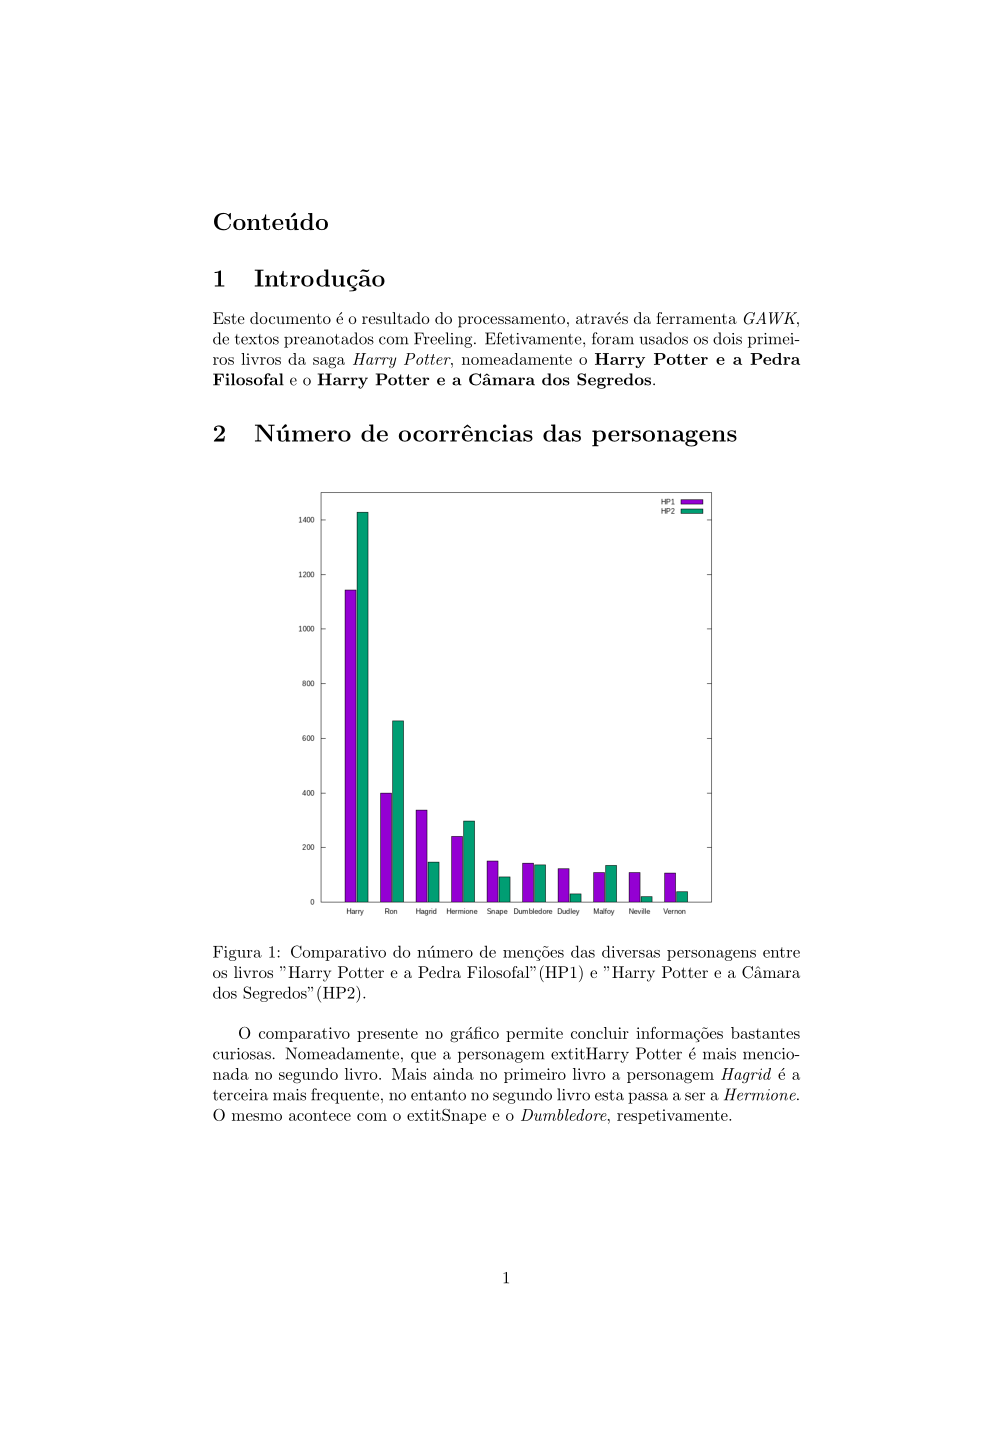
\includegraphics[width=1.3\linewidth]{grafico_pers.png}
	\end{subfigure}%
	\begin{subfigure}{0.5\textwidth}
		\centering
		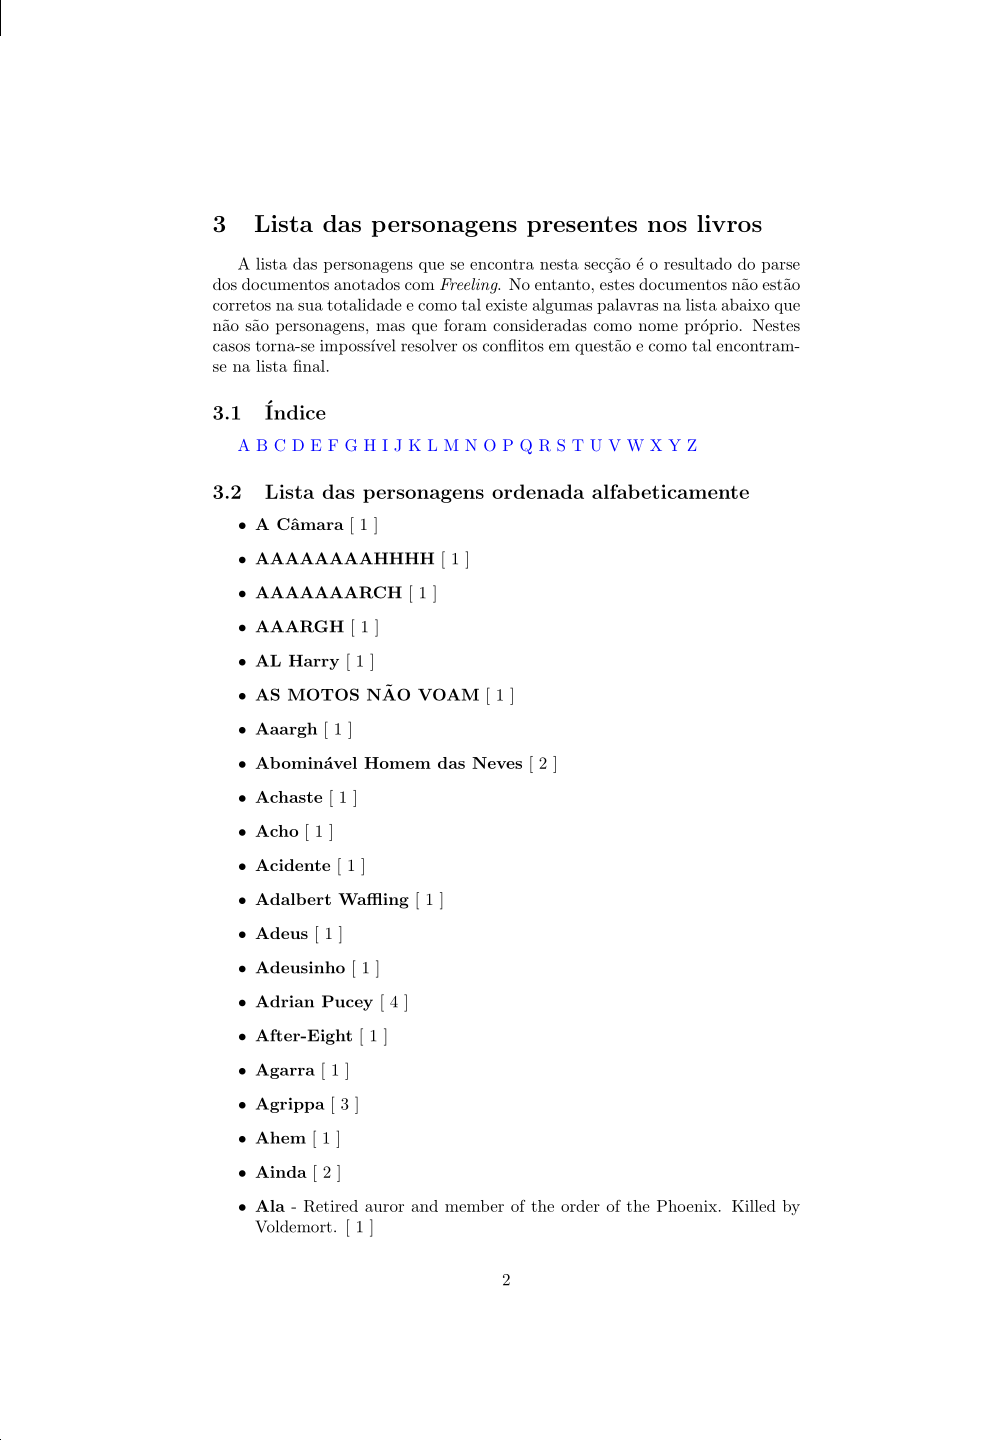
\includegraphics[width=1.3\linewidth]{list_pers.png}
	\end{subfigure}
	\caption{Relatório final.}
	\label{fig:relatorio_final}
\end{figure}

\newpage

%------------------------------------------------------------------------
\subsection{Lista dos verbos, substantivos, adjetivos e advérbios}

\hspace{3mm} Para a elaboração de uma lista dos verbos, substantivos, adjetivos e advérbios foi necessária mais uma vez uma análise em detalhe dos \emph{snapshots} disponibilizados.

\par Deste modo, observou-se que cada uma das categorias de palavras acima descritas se encontra definida segundo a sua classe gramatical na 3ª coluna de cada um dos extratos a analisar. Por consequência, procedeu-se ao desenvolvimento de uma expressão regular para cada um dos casos acima apresentados complementando sempre com a restrição de que o \emph{number of fields} terá de ser superior a 0, evitando assim erros no processamento da informação. Ainda dentro desta fase da análise da informação presente nos extratos, procede-se também ao tratamento da mesma, efetuando a substituição em cada um dos campos necessários dos caracteres \emph{\_} por espaços, tornando assim a sua leitura mais natural.

\begin{lstlisting}[language=Awk, caption=Preenchimento das estruturas de dados com o número de ocorrências de lemas e palavras.]
	NF > 0 && $4 ~ /^V.*/ { 
        gsub(/_/, " ", $3);
        gsub(/_/, " ", $2);
        verbos_lema[$3]++;
        verbos[$3][$2]++;
    }
\end{lstlisting}

\par Após todos os ficheiros serem processados e as frequências armazenadas nos respetivos arrays, procede-se então ao tratamento desta mesma informação para a sua apresentação.

\par Para uma melhor interpretação dos resultados obtidos, apresenta-se para além da listagem de todas as ocorrências de palavras e respetivo lema, um top 10 baseado no número de ocorrências. A construção deste passa por várias fases que irão ser descritas a seguir.

\par Primeiramente, são preenchidas estruturas auxiliares que irão albergar a informação respetiva aos tops de cada uma das categorias com as primeiras 10 ocorrências, sendo estas a informação base de comparação com os restantes resultados. Abaixo podemos ver o algoritmo utilizado para o caso das estruturas auxiliares de verbos, sendo o processo análogo para as restantes classes de palavras

\begin{lstlisting}[language=Awk, caption=Preenchimento inicial das estruturas de dados dos tops.]
	a = 0;
        for (i in verbos_lema){
            for (j in verbos[i]){
                if (a < 10){
                    top_verbos_palavra[a] = j;
                    top_verbos_lema[a] = i;
                    top_verbos[a] = verbos[i][j]; a++;
                }
                else break;
            }
        }
\end{lstlisting}


\par De seguida, as primeiras 10 ocorrências inseridas inicialmente serão ordenadas pelo número de ocorrências para que mais tarde, quando a restante estrutura de dados for percorrida, seja possível ser feita uma inserção ordenada no array top, evitando assim travessias adicionais quer das estruturas de dados extraídos, quer do próprio array de top. Na imagem apenas se encontra representado o caso de ordenação do array de verbos uma vez que para as restantes classes o processo é análogo.

\begin{lstlisting}[language=Awk, caption=Ordenação inicial da estrutura de dados top.]
	for (d = 0; d < 10; d++){
        for (b = d; b < 10; b++){
            if (top_verbos[d] < top_verbos[b]){
                temp = top_verbos[d];
                top_verbos[d] = top_verbos[b];
                top_verbos[b] = temp;

                temp = top_verbos_lema[d];
                top_verbos_lema[d] = top_verbos_lema[b];
                top_verbos_lema[b] = temp;

                temp = top_verbos_palavra[d];
                top_verbos_palavra[d] = top_verbos_palavra[b];
                top_verbos_palavra[b] = temp;
            }
        }
    }
\end{lstlisting}

\par Finalmente, são percorridas as estruturas de dados de cada uma das classes de palavras e, para cada uma das ocorrências, é verificado se essa mesma ocorrência se enquadra no cenário de top. Esta verificação consiste na tentativa da inserção da ocorrência efetuando a comparação com os dados presentes no momento no \textit{array} top e, no caso de esta ocorrência for maior do que algum dos dados já presentes no top, os elementos com frequência menor são movidos uma posição para a direita, sendo a ultima posição do \textit{array} descartado, e é inserida a nova ocorrência no local correto. Apenas é possível recorrer a este método de inserção uma vez que o array inicial se encontrava já ordenado.

\begin{lstlisting}[language=Awk, caption=Tentativa de inserção ordenada no \textit{array} top de cada uma das ocorrências de palavra.]
	for (n in verbos_lema){
            for (o in verbos[n]){

                for(i = 0; i < 10; i++){
                    if (top_verbos[i] < verbos[n][o]){
                        #SHIFT PARA A DIREITA
                        for(j = 9; j < i; j--){
                            top_verbos[j-1] = top_verbos[j];
                            top_verbos_lema[j-1] = top_verbos_lema[j];
                            top_verbos_palavra[j-1] = top_verbos_palavra[j];
                        }
                        top_verbos[i] = verbos[n][o];
                        top_verbos_lema[i] = n;
                        top_verbos_palavra[i] = o;
                        break;
                    }
                }

            }
        }
\end{lstlisting}

\par Para além dos tops descritos acima, será também apresentada a lista com todas as ocorrências, respetivo lema e frequência, ordenados alfabeticamente, para que o utilizador possa ter acesso ao relatório completo do número de ocorrências. Estas listas encontram-se também divididas segundo as classes acima referidas (verbos, adjetivos, advérbios e substantivos).
\par Para a apresentação desta lista completa de ocorrências, são utilizadas mais uma vez as estruturas de dados preenchidas inicialmente organizadas por lema e palavra mas, agora ordenadas alfabeticamente. Para esta ordenação, recorreu-se à função \emph{asorti}, que ordena \textit{arrays} com base no índice dos mesmos, como podemos ver abaixo.

\par Por forma a que a informação fosse apresentada da forma mais clara possível, o formato escolhido para a exportação dos dados foi o \emph{HTML}.
\par Para a construção dos ficheiros finais, é necessário seguir as regras de estruturação de um ficheiro deste formato. Para isso, irão ser explicitados os passos tomados.
\par Ainda na secção \emph{BEGIN}, é impressa a estruturação inicial do documento, bem como a definição do tipo de caracteres a utilizar, de modo a uniformizar o ficheiro. É definido também um titulo identificativo da classe da informação representada no ficheiro.

\begin{lstlisting}[language=Awk, caption=Inicialização da estruturação dos documentos \emph{HTML}.]
	 print "<html>\n<head><meta charset=\"UTF-8\"></head>\n<body>\n\n<h1 align=""\"center\""">Verbos</h1>" > "verbos.html"
\end{lstlisting}

\par Na próxima escrita para os ficheiros \emph{HTML}, são inicializadas as tabelas de tops e respetivos títulos, como podemos ver abaixo.

\begin{lstlisting}[language=Awk, caption=Inicialização da tabela e respetivo título.]
	print "<h2 align=""\"center\""">Top 10 Ocorrencias</h2>" > "verbos.html";
    print "\n<table align=""\"center\""" border='3'>\n\t\t" > "verbos.html"; 
    print "<tr bgcolor=""\"grey\""">\n\t\t<th>Lema</th><th>Palavra</th><th>Ocorrencias</th>\n\t</tr>" > "verbos.html"
\end{lstlisting}

\par Após toda a construção dos tops descrita acima, procede-se à exportação dos mesmos para a estrutura da tabela. Neste momento podemos já fechar a tabela dos tops, uma vez que já foi exportada toda a informação necessária.

\begin{lstlisting}[language=Awk, caption=Exportação dos dados dos verbos para a tabela top e exportação das tags de fecho da mesma. Análogo para as outras componentes.]
	for (b = 0; b < 10; b++){
                #print top_verbos[b], top_verbos_lema[b], top_verbos_palavra[b];
                print "<tr>\n\t<td>" top_verbos_lema[b] "</td><td>" top_verbos_palavra[b] "</td><td>"top_verbos[b]"</td>\n</tr>\n" > "verbos.html";
    }
    
    print "\t</table>" > "verbos.html";
\end{lstlisting}

\par De seguida, procede-se à inicialização da tabela que albergará toda as palavras e informação associada adicionando um título informativo e finalmente inicializando a tabela.

\begin{lstlisting}[language=Awk, caption=Inicialização da tabela completa de ocorrências para o caso específico dos verbos. Análogo para as outras componentes.]
    print "<h2 align=""\"center\""">Todas as ocorrencias de verbos</h2>" > "verbos.html";

    print "<table bgcolor=""\"#f2f2f2\""" align=""\"center\""" border='3'>" > "verbos.html"

    print "\t<tr bgcolor=""\"grey\""">\n\t\t<th>Lema</th>\n\t\t<th>Palavra</th>\n\t\t<th>Ocorrencias</th>\n\t</tr>" > "verbos.html"
\end{lstlisting}

\par Como foi referido acima, neste momento procede-se à exportação de cada uma das ocorrências para a respetiva tabela com o seguinte código.

\begin{lstlisting}[language=Awk, caption=Exportação de cada uma das ocorrências de palavra e respetivas informações associadas para a tabela completa de palavras.]
    asorti(verbos_lema, verbos_lema_sort); 
    for (i in verbos_lema_sort){
            asorti(verbos[verbos_lema_sort[i]], verbos_palavras);
            print verbos_lema_sort[i], ":" > "verbos.txt";

            for (a in verbos_palavras) conta++;

            #HTML
            print "\t<tr bgcolor=""\"#bfbfbf\""" align=""center"">\n\t\t<td rowspan="conta+1">"verbos_lema_sort[i]"</td>\n\t</tr>" > "verbos.html";

            for (j in verbos_palavras){
                    print  verbos_palavras[j], " -> ", verbos[verbos_lema_sort[i]][verbos_palavras[j]] > "verbos.txt";
                    #HTML
                    print "\t<tr>\n\t\t<td>"verbos_palavras[j]"</td>\n\t\t<td>"verbos[verbos_lema_sort[i]][verbos_palavras[j]]"</td>\n\t</tr>" > "verbos.html";
           }
           conta = 0;
    }
\end{lstlisting}

\par Para concluir, apenas será necessário fechar a tabela de ocorrências procedendo do seguinte modo.
\begin{lstlisting}[language=Awk, caption=Fecho da tabela que alberga a totalidade da informação.]
    print "</table>\n</body>\n</html>" > "verbos.html";
\end{lstlisting}

\subsection{Dicionário implícito no CORPORA}

\hspace{3mm} Pretende-se extrair dos ficheiros de texto uma lista de todos os seus \texttt{lemas} e, para cada \texttt{lema}, criar uma sub-lista de \texttt{palavras} e respetivos \texttt{pos} de modo a gerar um dicionário. Como tal, observando a estrutura dos dados, observa-se que se irá guardar informação dos segundo, terceiro e quarto campos.

\begin{figure}[!h]
    \centering
    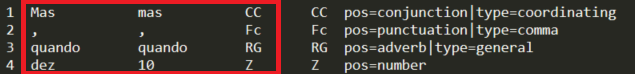
\includegraphics{dic1.png}
    \caption{Os campos que serão lidos serão os em destaque.}
    \label{fig:dic1}
\end{figure}

\par Neste caso o programa não necessita efetuar quaisquer ações previamente à leitura dos ficheiros, logo, não é executada nenhuma ação na secção \textit{BEGIN}.

\par Para que não ocorram erros de leitura de campos durante a execução do programa devido a linhas vazias, será necessário adicionar a condição de execução \texttt{NF > 0} em cada linha do ficheiro. Como se trata de um dicionário, será necessário filtrar todos os \texttt{lemas} correspondentes a pontuação (i.e. pontos, vírgulas, etc). Uma análise do formato \textit{Freeling} mostra que todos estes têm o \texttt{pos} \textbf{F} seguido de um ou mais carateres. \cite{Freeling} Como tal, outra condição de processamento de informação de cada linha será \texttt{\$4 !\~ \/F.+\/} . Quando é encontrada uma linha que passe a condição, o seu \texttt{lema} é guardado num \textit{array} associativo \textbf{dic\_palavras}, cujos índices são os próprios \texttt{lemas}. Cada \texttt{palavra} e \texttt{pos} de um determinado \texttt{lema} será, por sua vez, guardado num \textit{array} associativo bidimensional \textbf{dicionario}, cujos índices são o dado \texttt{lema} e a concatenação da \texttt{palavra} e \texttt{pos}, separados pelo carater \textit{SUBSEP}, nativo ao \textit{Gawk}.

\par No final da leitura dos ficheiros, procede-se à organização e armazenamento dos dados num novo ficheiro. É efetuado um \textit{asorti} do \textit{array} \textit{dic\_palavras} de modo a obter uma lista dos \texttt{lemas} ordenada alfabeticamente. Percorrendo o \textit{array} resultante \textbf{palavras}, efetua-se um \textit{asorti} a cada elemento \texttt{dicionario[palavras[i]]} para ordenar cada uma das \texttt{palavras} derivadas do respetivo \texttt{lema} por ordem alfabética, guardando-a no \textit{array} \textbf{definicoes}. Finalmente, efetua-se um \textit{split} de cada elemento de \textit{definicoes} para recuperar as \texttt{palavras} e \texttt{pos}.

\par Tendo planificado como se iria processar os dados, ponderou-se qual seria o melhor método de armazenamento dos mesmos. Decidiu-se guardar os dados do dicionário \textit{Corpora} em formato XML devido à sua capacidade de descrever informação com exatidão e sem ambiguidade e o facto de que o seu conteúdo é independente de formatação. Para tal, é necessário definir a estrutura do ficheiro que se pretende gerar. O ficheiro XML resultante será composto por uma \textit{tag} \textbf{dicionario}, que contém um conjunto \textit{tags} \textbf{termo}. Cada uma destas é composta por uma \textit{tag} \textbf{lema} que, como o nome sugere, contém um \texttt{lema} como atributo \textbf{id}, bem como um conjunto de \textit{tags} \textbf{palavra} que, por sua vez, guardam uma \texttt{palavra} como atributo \textbf{id} e o correspondente \texttt{pos}, na sua própria \textit{tag}.

\par De modo a manter a sintaxe do XML, é necessário certificar que não são passados carateres que possam ser mal interpretadas quando lidas após a sua geração. Neste caso, trata-se apenas do carater \&, que terá de ser substituído por "\&amp;". Como tal, antes da escrita de qualquer \texttt{lema} ou \texttt{palavra}, será efetuado um \textit{gsub} para certificar que a semântica do XML permaneça intacta.

\par Por fim, é de notar que a primeira linha de um ficheiro XML especifica o seu \textit{encoding}. Assim, a primeira linha escrita no ficheiro será a seguinte: \( <?xml version="1.0" ?> \).


\par Deste modo, o ficheiro resultante toma este aspeto:

\begin{figure}[!h]
    \centering
    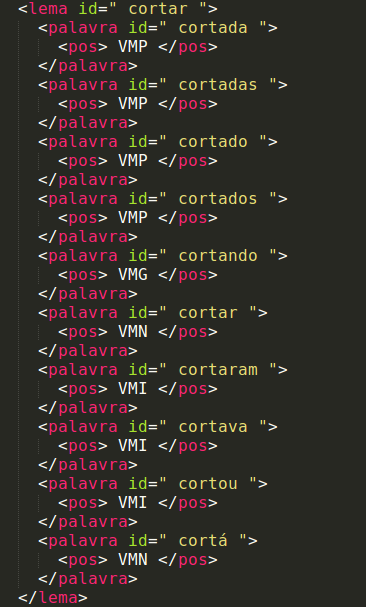
\includegraphics[width=3cm]{dic2.png}
    \caption{Exemplo do conteúdo do ficheiro resultante da execução do programa.}
    \label{fig:dic2}
\end{figure}

\newpage

%------------------------------------------------------------------------

\section{Conclusões e Sugestões}
\label{sec:5}
\hspace{3mm} Este projeto contempla inúmeras funcionalidades que o \textit{GAWK} fornece. Com ele foi possível processar registos de ficheiros, produzir ficheiros \textit{tex}, converter o formato dos dados, imprimir \textit{html} ou mesmo \textit{XML}.

Desta forma, com a ajuda da ferramenta mencionada anteriormente conseguiu-se produzir um relatório que analisa com algum pormenor as personagens dos dois primeiros livro da saga \textit{Harry Potter}. Mais ainda, foi possível extrair todos os verbos, adjetivos, substantivos e advérbios dos cinco ficheiros disponíveis e produzir um ficheiro \textit{html} de melhor compreensão e fácil análise. Além disso, foram aglomerados os lemas, palavras e o pos de cada palavra num ficheiro \textit{XML}, dicionário pronto a usar para trabalhos futuros.

No entanto, a informação presente nos documentos disponibilizados é bastante abrangente e diversa. Como tal, as funcionalidades aqui apresentadas podem ser melhoradas, ou novas podem ser acrescentadas, em iterações futuras do projeto. Desta forma, possíveis melhoramentos passariam por filtrar possíveis erros que existam no ficheiros base, para que esses não sejam carregados para o programas \textit{AWK}. Além disso, o XML produzido pode ser integrada numa componente gráfica, de forma a providenciar ao utilizador uma melhor interface na leitura do dicionário.

Neste projeto fica evidente o processo no qual, tendo ficheiros anotados com \textit{Freeling}, é possível extrair informação destes através de \textit{GAWK} e por fim converte-la para praticamente qualquer formato existente, nomeadamente, \textit{html}, \textit{\LaTeX} e \textit{XML}.


\newpage 

\begin{thebibliography}{3}

\bibitem{Awk}
Applying Minilanguages; Case Study: awk  
\hyperref[Awk]{http://www.faqs.org/docs/artu/ch08s02.html\#awk}

\bibitem{Aho}
The A-Z of Programming Languages: AWK  
\hyperref[Aho]{https://www.computerworld.com.au/article/216844/}

\bibitem{dataset} 
Potter Network: characters dataset,
\hyperref[dataset]{https://github.com/efekarakus/potter-network/blob/master/data/characters.csv}

\bibitem{Freeling}
FreeLing 4.0 User Manual
\hyperref[Freeling]{https://www.gitbook.com/book/talp-upc/freeling-4-0-user-manual/details}

\end{thebibliography}


\end{document}
